\chapter{Anonimato} \label{sect:AC}

\section{Canales Anónimos}

Los \textit{Canales Anónimos} permiten a los usuarios intercambiar mensajes sin revelar sus
identidades. Las aplicaciones son variadas y van desde votaciones, donde la identidad de los
votantes debe ser anónima, hasta bases de datos con información confidencial por su alta sensibilidad,
como bases de datos medicas.
Seguiremos la definición de canal anónimo de \cite{conf/pet/HeviaM08}, pues es lo suficientemente
general.\\
Consideremos la situación en que existen $n$ participantes, cuyas identidades son $P_{1},\ldots,P_{n}$,
que ejecutan una instancia de un protocolo $\pi$.
El conjunto de mensajes intercambiados entre $P_{1},\ldots,P_{n}$ en la ejecución de $\pi$ se puede
representar por una matriz $M$. Cada elemento de la matriz, $m_{ij}$,
es el multiconjunto de mensajes que envía algún participante $P_{i}$ a
otro participante $P_{j}$. Intuitivamente la comunicación con el
protocolo $\pi$ será anónima si ningún observador es capaz de obtener
más que ``cierta'' información de $M$. La información que el observador
sí puede obtener es una variable del modelo y lleva a considerar
distintos tipos de anonimato.\\
Consideraremos la ejecución de un protocolo en una configuración similar a UC, en que el adversario
es pasivo (no inyecta ni altera mensajes) y adicionalmente el ambiente recibe como parámetro la matriz
$M \in \mathcal{M}_{n \times n}(\mathcal{P}(\{0,1\}^{p(k)}))$, con $k$ el parámetro de seguridad y $p$
un polinomio. El ambiente pasa como parámetro a $P_i$ $i \in \{1, \ldots, n\}$ los mensajes
$\{(m_{i,j}, P_j)\}_{j=1}^n$, indicando que el mensaje $m_{i, j}$ es enviado por $P_i$ a $P_j$.
Nos centraremos en protocolos conocidos como \textit{protocolos de transmisión de mensajes}.

\begin{definicion}[Protocolo de trasmisión de mensajes]
Decimos que un protocolo $\pi$ es un protocolo de transmisión de mensajes si al ser ejecutado con entrada
$M$ para la salida de cada participante $P_i$ $i \in \{1, \ldots, n\}$ es el multiconjunto
$\uplus_{j=1}^n \{m_{i,j}\}$.
\end{definicion}

Definimos el experimento $\mathrm{Exp}_{\pi, \mathcal{A}}^{\mathcal{R}-anon}$, donde
$\mathcal{R} \subseteq \mathcal{M}_{n \times n}(\mathcal{P}(\{0,1\}^{p(k)}))^2$, en la figura \ref{exp_anon}.

\begin{definicion}
Decimos que un protocolo de transmisión de mensajes $\pi$ es $\mathcal{R}$-anónimo si para todo
adversario PPT $\mathcal{A}$ existe una función despreciable $\eta$ talque
$$2\cdot\Pr[\mathrm{Exp}_{\pi, \mathcal{A}}^{\mathcal{R}-anon}(k) = 1] - 1 \leq \eta(k)$$
\end{definicion}

Notemos que el adversario $\mathcal{A}$ solo puede elegir matrices $M_1, M_2$ tales que
$(M_1, M_2) \in \mathcal{R}$, de este modo $\mathcal{R}$ se puede usar para determinar la filtración
de información permitida al protocolo y con ello el tipo de anonimato. En efecto,
sea $f$ una función $f:\mathcal{M}_{n \times n}(\mathcal{P}(\{0,1\}^{p(k)})) \to I$, con I algún conjunto,
que llamaremos \textit{función de filtración de información}. 
Si por ejemplo $f(M) = \sum_{i, j} |m_{i,j}|$, el filtraje de información
correspondería al tamaño total de los mensajes intercambiados.
Si $\pi$ permite computar $f(M)$ al adversario, entonces trivialmente este puede distinguir
entre la ejecución de $\pi$ con una matriz $M_1$ y la ejecución de $\pi$ con otra matriz $M_2$
si elije $M_1$ y $M_2$ tales que $f(M_1) \neq f(M_2)$. Si definimos
$\mathcal{R} =  \{(M_1, M_2)| f(M_1) = f(M_2)\}$ entonces $\mathcal{A}$ ya no podrá efectuar este ataque,
y cualquier distinción entre la ejecución  de $\pi$ con $M_1$ y  $M_2$ dependerá de otro ``filtraje''
de información.\\
En \cite{conf/pet/HeviaM08} se definen tres funciones de filtración de información, estas son
$f_{\cup}, f_{\Sigma}, f_{\#}$ y se definen como sigue:
$$f_\cup(M) = \left(\biguplus_{j=1}^n \{m_{1,j}\}, \ldots, \biguplus_{j=1}^n \{m_{n,j}\}\right)$$
$$f_\Sigma(M) = \left(\sum_{j=1}^n |m_{1,j}|, \ldots, \sum_{j=1}^n |m_{n,j}|\right)$$
$$f_\#(M) = \sum_{i=1}^n \sum_{j=1}^n |m_{i,j}|$$
$f_\cup(M)$ corresponde al vector donde la componente $i$-ésima es el multiconjunto de mensajes
enviados por $P_i$, $f_\Sigma(M)$ corresponde al vector donde la componente $i$-ésima es el tamaño
en bits del total de mensajes enviados por $P_i$ y $f_\#(M)$ corresponde al tamaño total en bits
de mensajes enviados en el protocolo. Adicionalmente se define $f^T(M) = f(M^T)$ donde $M^T$ denota
la matriz $M$ transpuesta, y de ese modo $f^T_\cup(M)$ y $f^T_\Sigma(M)$ corresponden a vectores
donde el elemento $i$-ésimo es un valor calculado sobre los mensajes recibidos por $P_i$.\\
Adicionalmente en este trabajo definimos una nueva función de filtración de información,
$f_{\cup\cup}$ que viene dada por:
$$f_{\cup\cup}(M) = \biguplus_{i=1}^n \biguplus_{i=1}^n m_{i,j}$$
Cada función da lugar a una relación
$\mathcal{R}_f = \{(M_1, M_2 | f(M_1)=f(M_2))\}$, adicionalmente denotamos por
$\mathcal{R}_\star$ a $\mathcal{R}_{f_\star}$.
En \cite{conf/pet/HeviaM08} se definen diez relaciones dando lugar a diez tipos de anonimato, los
que se ilustran en la tabla y adicionalmente, con la función $f_{\cup\cup}$, definimos un nuevo
tipo de anonimato que llamamos \textit{Anonimato $f_{\cup\cup}$}.
\begin{table}
\begin{center}
\begin{tabular}{|l|c|}
\hline
Tipo de anonimato & Relación \\
\hline
\hline
Invinculabilidad débil & $\mathcal{R}_\cup \cap \mathcal{R}_\cup^T$ \\
\hline
Invinculabilidad del enviador & $\mathcal{R}_\Sigma \cap \mathcal{R}_\cup^T$ \\
\hline
Invinculabilidad del receptor & $\mathcal{R}_\cup \cap \mathcal{R}_\Sigma^T$ \\
\hline
Invinculabilidad & $\mathcal{R}_\Sigma \cap \mathcal{R}_\Sigma^T$ \\
\hline
Anonimato del enviador & $\mathcal{R}_\cup$ \\
\hline
Anonimato del receptor & $\mathcal{R}_\cup^T$ \\
\hline
Anonimato $f_{\cup\cup}$ & $\mathcal{R}_{\cup\cup}$\\
\hline
Anonimato del enviador fuerte & $\mathcal{R}_\Sigma$ \\
\hline
Anonimato del receptor fuerte & $\mathcal{R}_\Sigma^T$ \\
\hline
Anonimato del enviador y receptor & $\mathcal{R}_\#$ \\
\hline
Inobservabilidad & $\mathcal{M}_{n \times n}(\mathcal{P}(\{0, 1\}^{p(k)}))$ \\
\hline
\end{tabular}
\end{center}
\caption{Tipos de anonimato}
\label{tabla_anon}
\end{table}

\begin{figure}
\begin{centering}
\framebox{\begin{minipage}[t]{1\columnwidth}
El experimento $\mathrm{Exp}_{\pi, \mathcal{A}}^{\mathcal{R}-anon}(k)$ procede como
sigue:
\begin{enumerate}
    \item Escoger $b \in_R \{0, 1\}$ y ejecutar $(M_0, M_1) \leftarrow \mathcal{A}(k)$
    \item Si $(M_0, M_1) \notin \mathcal{R}$ retornar 0
    \item Ejecutar $\pi$ con la matriz $M_b$ y adversario $\mathcal{A}$ hasta que $\mathcal{A}$
          retorne un bit $b_\mathcal{A}$
    \item Si $b = b_\mathcal{A}$ retornar 1, de lo contrario retornar 0.
\end{enumerate}
\end{minipage}}
\end{centering}
\caption{El experimento $\mathrm{Exp}_{\pi, \mathcal{A}}^{\mathcal{R}-anon}$}
\label{exp_anon}
\end{figure}

Notemos que la nueva noción de anonimato es más fuerte que las nociones de anonimato del receptor/enviador.
En efecto, solo hay que notar que para cualquier par de matrices $f_\cup(M_1) = f_\cup(M_2)$ implica que
$f_{\cup\cup}(M_1) = f_{\cup\cup}(M_2)$, por lo tanto $\mathcal{R}_\cup \subseteq \mathcal{R}_{\cup\cup}$
y $\mathcal{R}_\cup^T \subseteq \mathcal{R}_{\cup\cup}$.

\section{Primitivas para Canales Anónimos}

Variadas primitivas útiles para implementar canales anónimos han sido propuestas en la literatura. A continuación
revisamos cuatro primitivas para canales anónimos.

\subsection{Redes de Mezcla o \textit{Mix-nets}}
El estudio moderno protocolos de canales anónimos comenzó en \cite{journals/cacm/Chaum81} con las Redes
de Mezcla o \textit{mix-nets}. En una mix-net el vector $v_0$ formado por los mensajes encriptados de todos
los participantes es enviado a través de una serie de \textit{mixers} (en español mezcladores). Cada
mixer $M_i$ realiza una operación en el vector de textos cifrados $v_{i-1}$, obteniendo nuevos textos cifrados
$v'_{i-1}$, y envía una
permutación aleatoria de los nuevos textos cifrados $v_i = \pi(v'_{i-1})$ al siguiente mixer.
La operación que cada mixer realiza debe ser tal que permite ocultar la permutación que efectuó el mixer.
Finalmente el último mixer publica una permutación del vector de mensajes $\pi(m_1, \ldots, m_n)$ de los
participantes. En la figura \ref{fig:mix-net} se puede ver un diagrama de una mix-net.\\

\begin{figure}[hp]
    \centering
    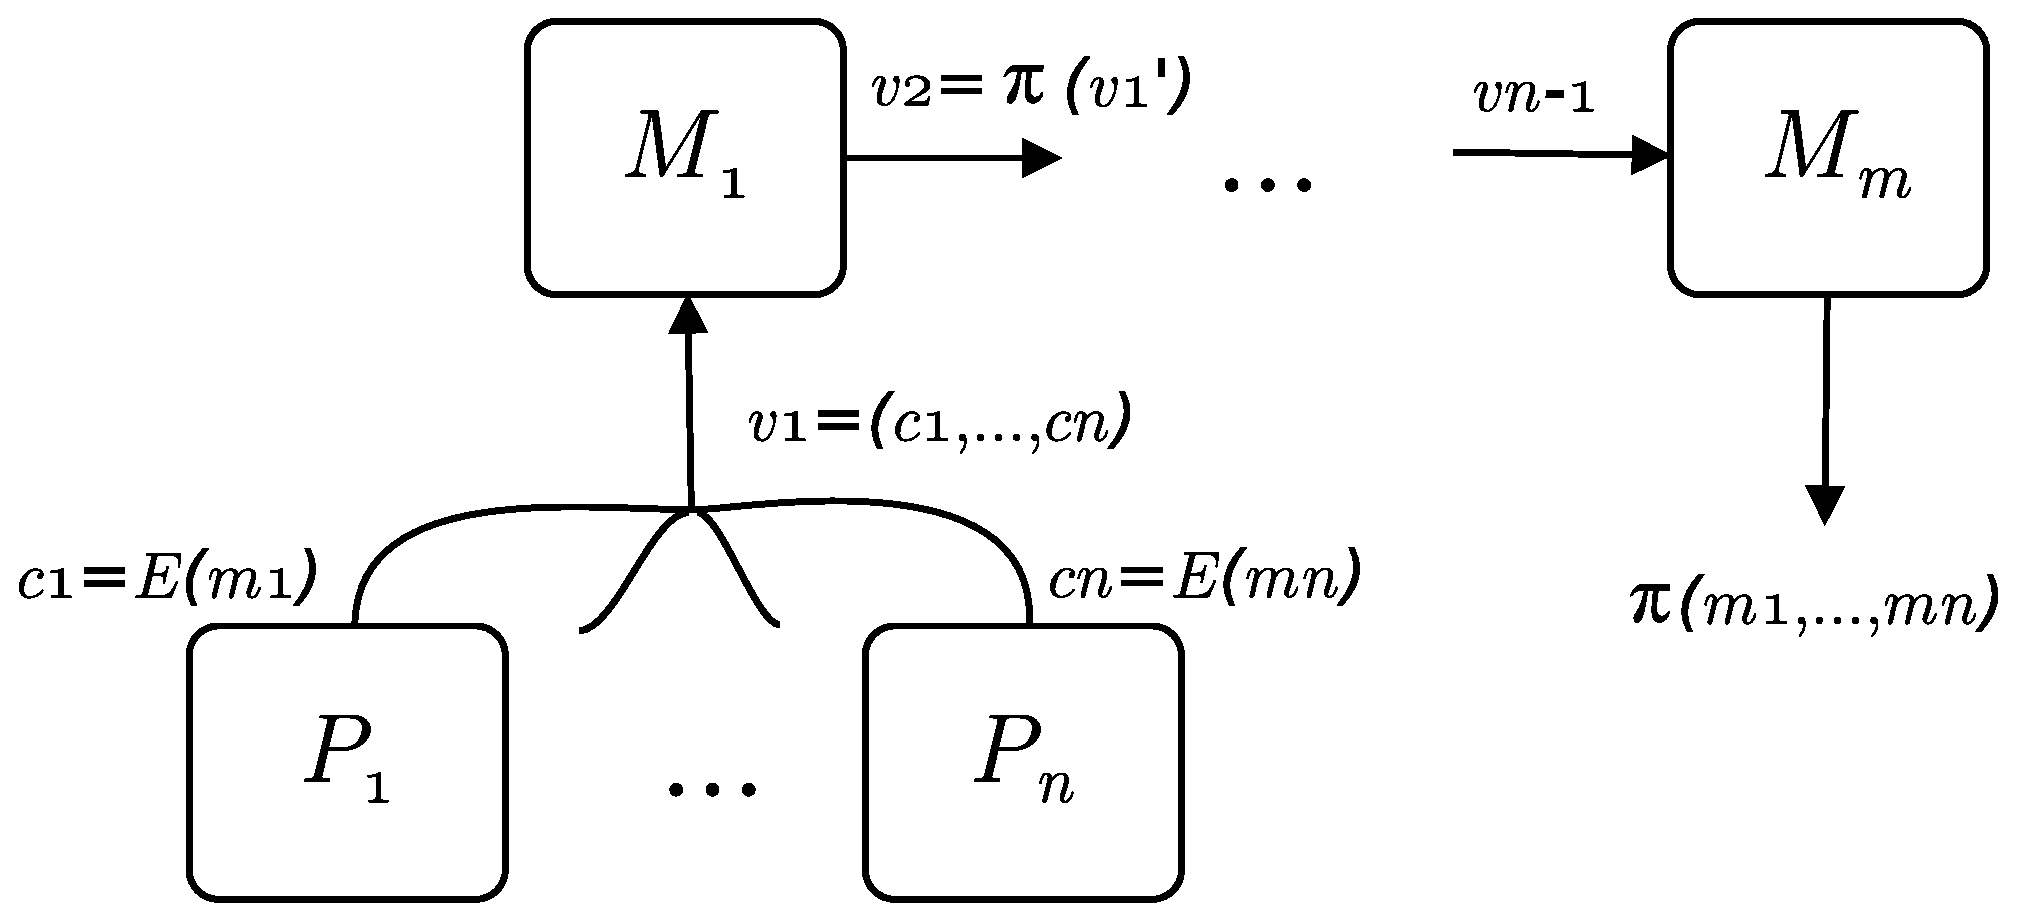
\includegraphics[width=0.7\textwidth]{figs/mixnet}
    \caption{Diagrama de una mix-net}
    \label{fig:mix-net}
\end{figure}


Las mix-nets se pueden clasificar en dos, según el tipo de operación que cada mixer realiza en los textos
cifrados: mix-nets reencriptantes y mix-nets desecncriptantes.

\subsection{Mix-nets reencriptantes}

En las mix-nets reencriptantes los Mixers permutan
aleatoriamente cada vector de mensajes y re-encriptan los textos planos.
Consideremos un esquema de encriptación asimétrico $\mathcal{E} = (K, E, D)$ y fijemos
una clave pública $pk$; entonces
una re-encriptación
corresponde a aplicar una función $\rho_{pk}:C\times R\to C$, con $C$ el
espacio de textos cifrados, tal que para todo $m, r, r', c$ tales que $c =  E_{pk}(m, r)$ y
$r \neq r'$:

$$D_{sk}(\rho_{pk}(c, r')) = m \quad \textrm{y además } \rho_{pk}(c, r') \neq c$$

En otras palabras la función $\rho$ cambia la aleatoriedad de un texto
cifrado.
Al cambiar la aleatoriedad y si  $\mathcal{E}$ es un esquema de encriptación seguro (IND-CPA)
no es posible para ningún adversario correlacionar las entradas y salidas de un mixer.

Un ejemplo de esquema de encriptación en el cual es posible reencriptar
los textos cifrados es ElGamal. Se puede implementar un algoritmo de reencriptación para
ElGamal usando que $E_{y}(m,r)\cdot E_{y}(m',r') = E_{y}(m \cdot m',r+r')$ (es homomórfico). En efecto:

$$ E_{y}(m,r) \cdot
    E_{y}(m',r')
=
(g^{r} \cdot g^{r'},
 y^{r} \cdot m \cdot y^{r'} \cdot m')
=
(g^{r+r'},
 y^{r+r'}m \cdot m') $$

Por lo tanto

$$ E_{y}(m,r) \cdot E_{y}(m',r') = E_{y}(m \cdot m', r+r')$$


Usando lo anterior es posible construir $\rho$ tomando $m'=1$, de este
modo

$$\rho_{y}(E(m,r),r') = E_{y}(m,r) \cdot E_{y}(1,r') = E_{y}(m,r+r')$$

Una desventaja de un esquema de encriptación que permite re-encriptación
como ElGamal es que para ocupar $\rho$ es necesario conocer la clave pública
de quien encriptó del emisor del mensaje. En el contexto de una mix-net esto
significaría que cada mixer debería primero obtener la clave de cada
enviador, lo cual puede resultar impráctico.
En \cite{GolleEtAl04}
proponen un esquema de encriptación en el cual no es necesario conocer
las claves públicas de los enviadores. Dicha propiedad la llaman Universal
Re-encryption y para obtenerla en un esquema basado en ElGamal básicamente
adjuntan en el texto cifrado lo necesario para homomorficamente cambiar
la aleatoriedad del texto cifrado. El esquema propuesto en \cite{GolleEtAl04}
esta compuesto por los algoritmos $(K,E,D,\rho)$ donde

$$K(k)=(x,y),\quad x\in_{R} G_{q},  y=g^{x}$$


$$E_{y}(m,(k_{0},k_{1}))=[(g^{k_{0}},y^{k_{0}}\cdot m);(g^{k_{1}},y^{k_{1}})]$$


$$D_{x}([(u,v);(\alpha,\beta)])=\frac{v}{u^{x}}$$


Notemos que la segunda componente de $E_{y}(m,(k_{0},k_{1}))$ (esto es $g^{k_1}$ y $y^{k_1}$)
es la encriptación de $1$ bajo la clave pública $y$ y aleatoriedad
$k_{1}$, entonces $\rho$ sigue esencialmente igual, salvo que no es necesario
conocer la clave pública. En efecto

$$
\rho([(u,v);(\alpha,\beta)],(k_{0},k_{1}))=
[(u\cdot \alpha^{k_{0}}, v\cdot \beta^{k_{0}});
 (\alpha^{k_{1}},\beta^{k_{1}})]
$$

\subsection{Mixnet con desencriptación}

En estos protocolos los Mixers desencriptan parcialmente los textos
cifrados y los permutan aleatoriamente, de modo que finalmente se
obtiene una permutación de los textos planos originales.\\
Una forma de implementar una mixnet con reencriptación es usando un
esquema de encriptación semánticamente seguro
$\mathcal{E}=(K,E,D^{dist},D)$. Para enviar un texto plano $m_{i}$ un enviador
$P_{i}$  encriptará $m_{i}$ bajo una clave
pública $pk$, cuya correspondiente clave privada es una función $f$
de las claves privadas de los Mixers $\{sk_{i}\}_{i=1}^{N}$.
Cada mixer $M_{k}$ toma un vector
de textos cifrados $(v_{1},v_{2}\ldots,v_{M})$ y desencripta parcialmente cada
texto cifrado con su clave secreta $sk_{k}$, de modo talque si nos restringimos
a vectores de textos cifrados de tamaño 1 el aporte
total de los mixers es:

\[
D_{sk_{1}}(D_{sk_{2}}(\ldots D_{sk_{N}}(E_{pk}(m,r)\ldots))=D_{f(sk_{1},sk_{2},\ldots,sk_{N})}(m)=m\]

Adicionalmente cada mixer $M_{i}$ escoge una permutación al azar
$\pi\in_{R}\Pi_{M}$, con $\Pi_{M}$ el conjunto
de todas las permutaciones de $\{1,\ldots,M\}$, y la aplica al vector
de textos cifrados parcialmente desencriptados para retornar otro
vector $(D_{sk_{i}}(v_{\pi^{-1}(1)}),D_{sk_{i}}(v_{\pi^{-1}(2)}),\ldots,D_{sk_{i}}(v_{\pi^{-1}(i)}))$.

\subsubsection{Mixnet de Wikstr\"om}

Para realizar nuestro protocolo (capítulo \ref{cap:protocolo}) utilizaremos la mixnet
UC-segura propuesta por Wikstr\"om en \cite{Wikstrom04a}. Básicamente a mixnet de Wikstr\"om's
procede como sigue:

\begin{enumerate}

\item Cada enviador $P_i$ espera por las claves públicas de los mixers y computa el producto
      de todas las claves públicas $y = \prod_{i=1}^k y_i$. Luego cada enviador encripta su mensaje
      con la clave pública $y$, publica el texto cifrado en una \textit{pizarra pública}
      \footnote{Una funcionalidad ideal $\mathcal{F}_{BB}$ que se comporta como una pizarra visible por todos
      los participantes y donde todos pueden escribir. Vista de otra forma, es una funcionalidad que permite
      hacer broadcast a todos los participantes.}
      y prueba que es un texto cifrado válido usando un protocolo ZKP.
\item Cada mixer $M_j$ $j\in{1, \ldots, k}$ descarta todos los textos cifrados que no son válidos.
      Luego, para $l = 1, \ldots, k$ si $l = j$ el mixer $M_l$ desencripta parcialmente la lista
      de textos cifrados obtenida de la pizarra pública, les aplica una permutación escogida al azar,
      publica la lista en la pizarra pública y prueba usando un protocolo ZKP que la lista publicada
      es una reencriptación de una permutación aleatoria de la lista anterior.
      Si $l \neq j$ el mixer $M_j$ debe chequear que la permutación publicada por $M_l$ es valida.
      Finalmente el mixer con índice mayor ordena la lista de textos planos resultantes de la
      desencriptación conjunta, y publica la lista.

\end{enumerate}

Adicionalmente, para fines de este trabajo, modificamos la mixnet de \cite{Wikstrom04a} para que el protocolo
no empiece a menos que haya una cantidad mínima de mensajes $\kappa$. La modificación se puede ver en 
la figura \ref{func:F_MN}. 

En \cite{mnCompleto} se muestra que este protocolo UC-realiza a la funcionalidad ideal $\mathcal{F}_{MN}$,
definida en la figura \ref{func:F_MN}, en el modelo $\mathcal{F}_{KG}$-híbrido. 

\begin{teorema}
El protocolo de \cite{Wikstrom04a} UC-realiza a la funcionalidad ideal $\mathcal{F}_{MN}$
en el modelo $\mathcal{F}_{KG}$-híbrido con respecto a adversarios estáticos y bajo DDH en un grupo
$G_q$.
\label{teo:mn}
\end{teorema}

Notamos que con la modificación, si bien se generaliza a la mixet de \cite{Wikstrom04a}, el teorema anterior
se sigue teniendo. En efecto si $\mathcal{C}_{Env}$ es el conjunto
de todos los ambientes y $\mathcal{C}_{Adv}$ es el conjunto de todos los adversarios, entonces el conjunto
de ambientes y adversarios $\mathcal{C}_{\kappa}$ para los que la cantidad de mensajes enviados a la mixnet
es mayor que $\kappa$ es claramente subconjunto de $\mathcal{C}_{Env}\times\mathcal{C}_{Adv}$. Por lo tanto
para cada $\mathcal{Z}$ y $\mathcal{A}$ tales que $(\mathcal{Z}, \mathcal{A}) \in \mathcal{C}_\kappa$ debe
existir un simulador $\mathcal{S^{Z, A}}$ talque el $\mathcal{Z}$ no distingue entre el mundo real e el
mundo ideal.

\begin{figure}
\begin{centering}
\framebox{\begin{minipage}[t]{1\columnwidth}
La funcionalidad ideal $\mathcal{F}^\kappa_{MN}$ corriendo con mixers $M_{1}, \ldots, M_{k}$, enviadores
$P_{1}, \ldots, P_{N}$, y adversario ideal $\mathcal{S}$: 
\begin{enumerate}
    \item Inicializar una lista $L = \emptyset$, conjuntos $J_P =  \emptyset$ y $J_M = \emptyset$ y
          variable $c = 0$.
    \item Si $(P_{i}, \mathtt{Send}, m_{i})$  $m_{i} \in G_q$ es recibido desde $\mathcal{C_I}$.
          Si $i\notin J_P$, hacer $J_P \leftarrow J_P \cup \{i\}$, $c \leftarrow c+1$, adjuntar
          $m_i$ a la lista $L$. Luego enviar $(\mathcal{S}, P_i, \mathtt{Send})$ a $\mathcal{C_I}$.
    \item Supongamos que $(M_{j}, \mathtt{Run})$ es recibido desde $\mathcal{C_I}$. Hacer
          $J_M \leftarrow J_M \cup \{j\}$. Si $|J_M | \geq k/2$ y $c \geq \kappa$, luego ordenar la
          lista lexicográficamente para formar una lista $L'$, y enviar
          $((\mathcal{S}, M_{j}, \mathtt{Output}, L'), \{M_l , \mathtt{Output}, L'\}_{l=1}^{k})$ a
          to $\mathcal{C_I}$. De lo contrario, enviar a $\mathcal{C_I}$ la lista
          $(\mathcal{S}, M_{j}, \mathtt{Run})$
\end{enumerate}
\end{minipage}}
\end{centering}
\caption{La funcionalidad ideal $\mathcal{F}_{MN}$}
\label{func:F_MN}
\end{figure}

\subsection{Anonimous Broadcast o DC-nets}

A diferencia de las mixnets, las DC-nets, propuestas por Chaum en
\cite{journals/joc/Chaum88}, no son interactivas. No es necesaria
la existencia de otros participantes mas que los enviadores y receptores,
por el contrario en las mixnets se necesita que los mixer manipulen
los textos cifrados antes de que puedan ser leídos por los receptores.
Cada enviador $P_{i}$ publica un vector de textos cifrados
$c_{i}=((\delta_{1}(m_{i},r_{i})\cdot c'_{i,1},\ldots,\delta_{m}(m,r_{i})\text{·}c'_{i,n})$
con $r_{i}\in0^{\ell_{i}}10^{m-\ell_{i}}$, $\ell_i \in \{1, \ldots m\}$ distinto para cada
$i$ y:
\[
\delta_{k}(m,r)=\begin{cases}
m & r[k]=1\\
1 & r[k]=0\end{cases}\quad\forall i\in\{1,\ldots,n\}\]


\[
\prod_{i=1}^{n}c'_{i,j}=1\quad\forall j\in\{1,\ldots,n\}\]


\[
\ell_{i}\neq\ell_{j}\mbox{ si }i\neq j\]


Posteriormente es posible obtener una permutación el vector $(\prod_{i=1}^{n}c{}_{i,j})_{j=1}^{n}$,
que corresponde a una permutación del vector $(m_{i})_{i=1}^{n}$.
Si la distribución que sigue $c_{i}$ es indistinguible de la que
sigue $m_{i}\text{·}c_{i}$ $\forall i$, entonces es imposible para
un adversario identificar al autor de algún texto plano.

